\chapter{Proiectare de detaliu și implementare}
\pagestyle{fancy}

Acest capitol prezinta in detaliu solutia propusa pentru un sistem de monitorizare a temperaturii si a umiditatii. Aceasta include protocoalele de 
comunicatie utilizate, limbajele de programare si arhitecturi de abstractizare.

Arhitectura generala a sistemului este compusa din 5 componente pricipale interconectate pentru a crea o retea bine definita si cu o flexibilitate
ridicata:
\begin{enumerate}
	\item Aplicatie Android
	\item MQTT Broker
	\item Server
	\item Baza de date
	\item Senzor
\end{enumerate}

\

Figura \ref{fig:ArhitecturaGenerala} prezinta arhitectura generala a sistemului continand modulele principale ale acestuia si protocoalele de comunicatie 
dintre acestea.
\begin{figure}[H]
    \centering
    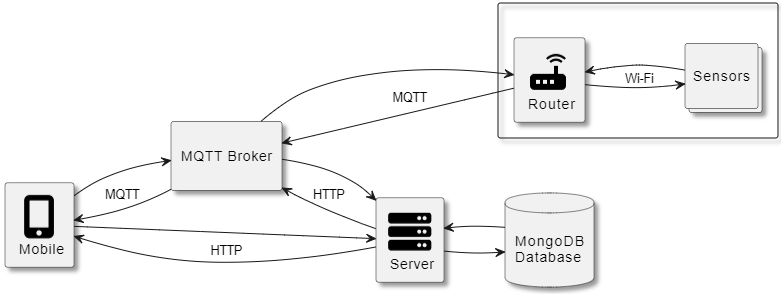
\includegraphics[scale=0.72]{figs/ArhitecturaGenerala.png}
    \caption{Arhitectura generala a proiectului}
    \label{fig:ArhitecturaGenerala}
\end{figure}

In subcapitolele urmatoare va fi descris in mod detaliat fiecare modul al sistemului si protocoalele de comunicatie utilizate pentru comunicarea dintre 
acestea.

\section{Aplicatia Android}\label{sec:pi_appandroid}
Aplicatia Android reprezinta interfata cu utilizatorul oferindui acestuia un mod usor de a gestiona mai multi senzori si de a monitoriza datele venite de la
acestia. Este scrisa in limbajul de programare Java si ruleaza pe sistemul de operare Android. Proiectul este scris in mediul de dezvoltare integrat Android 
Studio IDE.

In sistemul de operare Android clasele care definesc o interfata grafica sunt denumite activitati. La deschiderea aplicatiei este deschis firul de executie principal 
care are sarcina de a afisa interfetele grafice si de a gestiona actiunile utilizatorului, de exemplu, apasare de buton. Fiecare clasa de tip activitate extinde 
clasa AppCompatActivity care ofera componente pentru afisarea grafica si metode callback pentru gestionarea navigarii intre mai multe activitati. 

Aplicatia este compusa din 2 activitati principale si cateva secundare:
\begin{enumerate}
	\item ActivityWelcome - reprezinta activitatea care este afisata la deschiderea aplicatiei.
	\item ActivitySensor - reprezinta activitatea care este afisata atunci cand utilizatorul selecteaza un senzor din lista.
	\item ActivityInstall - reprezinta un grup de activitati secundare afisate atunci cand utilizatorul instaleaza un senzor nou. Fiecare dintre aceste 
	activitati reprezinta un pas din procesul de instalare.
\end{enumerate}

\

Figura \ref{fig:AndroidClassDiagram} prezinta diagrama de clase a aplicatiei Android.
\begin{figure}[H]
    \centering
    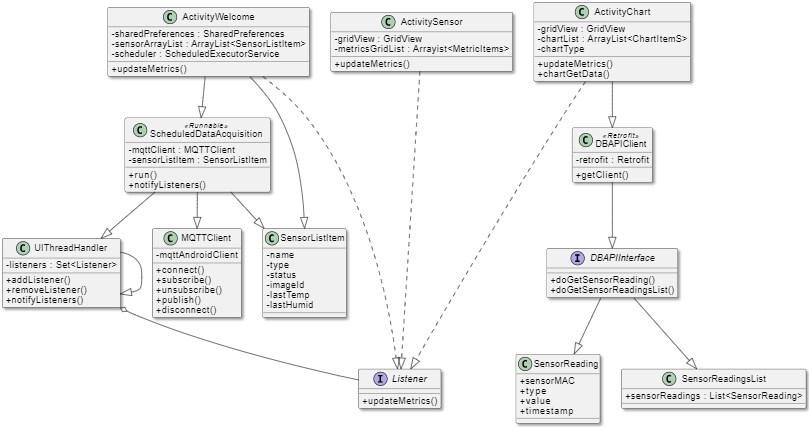
\includegraphics[scale=0.64]{figs/AndroidClassDiagram.png}
    \caption{Arhitectura generala a proiectului}
    \label{fig:AndroidClassDiagram}
\end{figure}

La incarcarea primei activitati care este afisata pe ecranul dispozitivului mobil, numita ActivityWelcome, se extrage din memorie o lista de senzori care au fost 
instalati in prealabil. Daca nu exista senzori instalati, aceasta lista nu va contine elemente. Lista este parcursa si pentru fiecare senzor este pornit un nou 
fir de executie periodic. Acest fir de executie are rolul de a gestiona conexiunea cu modulul MQTT Broker pentru senzorul respectiv, iar periodicitatea 
acestuia perimite verificarea si reincercarea conexiunii la un interval fix de timp. Apoi aceasta lista este afisata in interfata grafica. Fiecare element din lista 
contine: denumirea senzorului, tipul de senzor, statusul conexiunii si o imagine reprezentativa a senzorului.

Pentru memorarea senzorilor installati este utilizata biblioteca SharedPreferences. Aceasta contine rutine pentru salvarea datelor intr-un fisier din memoria 
dispozitivului mobil intr-un format de forma (cheie, valoare). Primul camp din acest fisier reprezinta numarul de senzori salvati, iar campurile ce urmeaza 
reprezinta senzorii instalati. Aceasta biblioteca este potrivita pentru memorarea datelor sub forma (cheie, valoare) si pentru compatibilitatea cu versiuni mai 
vechi de Android, spre deosebire de alte biblioteci precum DataStore care sunt potrivite pe seturi de date complexe si functioneaza doar in versiunile mai noi de 
Android.

Pentru firele de executie periodice este utilizata biblioteca ScheduledThreadPoolExecutor. Acesasta permite crearea unui grup de fire de executie care se executa
in paralel, spre deosebire de biblioteca Timer care are un singur fir de executie, iar o sarcina de durata mai lunga poate intarzia alte sarcini care asteapta 
executia. De asemenea, in cazul unei erori, doar sarcina in care a aparut eroarea va fi oprita, celelalte sarcini fiind executate in mod obisnuit. Aceasta 
biblioteca ofera siguranta continuarii executiei aplicatiei in cazul unei erori izolate.

La selectarea de catre utilizator a unui senzor din lista afisata este deschisa o noua activitate, numita ActivitySensor, iar la atingerea butonului de adaugare a unui 
nou senzor este deschisa prima activitate din grupul de activitati specifice instalarii. Pentru navigarea la o noua activitate si pentru transferarea de informatii intre 
activitati este utilizata clasa Intent. Aceasta clasa reprezinta o descriere abstracta a unei operatii. Cea mai semnificativa utilizare a acesteia este pentru operatia de 
deschidere a unei noi activitati. Pentru aceasta operatie se apeleaza functia startActivity() care primeste ca parametru o instanta a clasei Intent care contine informatiile 
necesare pentru ca operatia sa fie executata. Informatii precum activitatea parinte si activitatea care urmeaza a fi executata sunt necesare, iar in plus pot fi adaugate 
informatii care sa fie transferate catre activitatea copil utilizant functia putExtra() care primeste ca parametru o structura de tipul (cheie, valoare).

Pentru fiecare fir de executie specific unui senzor se creaza o instanta a clasei ScheduledDataAcquisition care implementeaza interfata runnable si executa periodic o rutina 
in care se verifica daca senzorul este conectat la modulul MQTT Broker. La prima executie senzorul este considerat deconectat si se executa rutina de conectare. 
Aceasta rutina utilizeaza clasa MQTTClient care ofera metodele necesare realizarii si gestionarii conexiunii cu modulul MQTT Broker. Pentru realizarea conexiunii se 
executa metoda connect a clasei MQTTClient care primeste ca paramterii 2 rutine callback. Aceste rutine definesc actiuni ce sunt executate atunci cand au loc 
diferite evenimente in tranzactionarea cu modulul MQTT Broker. Mai jos sunt enumerate cele mai importante astfel de evenimente:
\begin{itemize}
	\item Connectarea cu success la modulul MQTT Broker - cand are loc acest eveniment se executa rutina de subscriere pentru receptionarea in timp real a datelor de la 
	senzor.
	\item Pierderea conexiunii - acest eveniment va modifica statusul conexiunii din lista de senzori a-i activitatii ActivityWelcome si din ActivitySensor.
	\item Receptia unui mesaj - acest eveniment va apela metoda notifyListeners() a obiectului UIThreadHandler care va actualiza ultima valoare de temperatura si 
	umiditate afisata in activitatile ActivityWelcome si ActivitySensor. De asemenea, acest eveniment va verifica si statusul conexiunii senzorului si il va schimba 
	daca este cazul.
\end{itemize}

Clasa MQTTClient utilizeaza o instanta a clasei MqttAndroidClient oferita de biblioteca eclipse.paho.mqttv3 care reprezinta o implementare asincrona a 
al unui client al protocolului MQTT si are rolul de a gestiona impachetarea messajelor in formatul protocolului MQTT si tranzactionarea acestora cu un server MQTT. De asemenea, 
clasa MQTTClient defineste rutine de gestionare a exceptilor ridicate de obiectul MqttAndroidClient in cazul unei erori. 

Clasa UIThreadHandler are rolul de a efectua modificari in interfetele grafice de pe un fir de executie extern. Clasele de tip activitate sunt executate pe un fir de executie 
care are rolul strict de a raspunde la actiunile utilizatorului si doar acest fir de executie poate face modificari in interfata grafica, iar interogarea bazei de date sau 
receptionarea de date de la modulul MQTT sunt executate pe fire de executie diferite. Aceasta clasa realizeaza transferul de date sau evenimente care necesita modificarea 
interfetei grafice si care au fost primite pe un fir de executie extern catre firul de executie al interfetei grafice. Pentru a realiza acest transfer, instanta clasei  
UIThreadHandler mentine o lista de clase de tip Listener. Activitatile AvtivityWelcome si ActivitySensor sunt clase de tip Listener, deoarece implementeaza interfata 
Listener si metoda updateMetrics() a acesteia, iar la creare se inregistreaza in lista de obiecte Listener mentinuta de instanta UIThreadHandler. Fiecare activitate 
defineste in metoda updateMetrics() ce anume va fi modificat in interfata grafica. Atunci cand sunt receptionate date de la modulul MQTT Broker, se executa metoda 
notifyListeners() a obiectului UIThreadHander. Aceasta metoda parcurge lista de clase de tip Listener si pentru fiecare apeleaza metoda updateMetrics(). Aceasta metoda nu este 
apelata direct, ci prin obiectul Handler care primeste ca parametru o rutina de tip Runnable si care este pus intr-o coada de executie a interfetei grafice.

La selectarea unui element din lista de senzori afisata in activitatea ActivityWelcome este creata activitatea ActivitySensor. Rolul acesteia este de a prezenta informatiile 
senzorului selectat si datele de temperatura si umiditate ale acestuia sub forma grafica si sub forma a 2 campuri care contin doar ultima valoare receptionata. La creare 
se citeste din obiectul Intent primit de la activitatea ActivityWelcome informatiile senzorului intr-un obiect SensorListItem, se afiseaza informatiile senzorului in 
interfata grafica, se initializeaza graficele de temperatura si umiditate si se interogheaza baza de date pentru valorile din ultimele 10 minute. La primirea valorilor 
citite din baza de date, acestea sunt scrise in graficul de temperatura, respectiv umiditate. Daca nu exista date in ultimele 10 minute inseamna ca senzorul nu este conectat, iar 
statusul acestuia este modificat corespunzator. 

Pentru interogarea bazei de date este utilizata biblioteca Retrofit a carei functionalitate teoretica este descrisa in sectiunea \ref{sec:retrofit}. Pentru implementarea 
rutinelor de interogare a bazei de date utilizand aceasta biblioteca sunt utilizate urmatoarele clase din figura \ref{fig:AndroidClassDiagram}:
\begin{itemize}
	\item Clasa DBAPIClient - are rolul de a crea un obiect de tip Retrofit. Pentru crearea acestuia sunt necesare: adresa URL a server-ului, un obiect GsonConverterFactory 
	pentru convertirea automata a datelor si o instanta a clasei OkHttpClient.
	\item Interfata DBAPIInterface - declara metodele pentru interogarea bazei de date utilizand adnotari.
	\item Clasa SensorReading - este o clasa model care contine campurile receptionate in raspunsul metodei doGetSensorReading().
	\item Clasa SensorReadingsList - este o clasa model care contine o lista de obiecte de tip SensorReading. Aceasta lista reprezinta raspunsul metodei doGetSensorReadingsList().
\end{itemize}

La initierea unei interogari a bazei de date se obtine obiectul Retrofit utilizand metoda getClient() a clasei DBAPIClient. Se apeleaza metoda create() a obiectului Retrofit care 
primeste ca parametru interfata DBAPIInterface, iar pe baza acestei interfete, Retrofit va genera automat o clasa care contine implementarea metodelor declarate in aceasta. 
Utilizand instanta clasei creata automat se acceseaza una din metodele acesteia si se pune intr-o coada de transmisie impreuna cu o metoda callback care va fi executata cand 
este receptionat raspunsul de la server sau cand expira timpul de asteptare. La receptionarea raspunsului, biblioteca Retrofit va interpreta datele receptionate in format GSON 
bazat pe clasa model specifica metodei care s-a executat si va crea un obiect de acest tip. In metoda callback se citeste obiectul si se adauga valorile de temperatura si 
umiditate in graficul respectiv fiecareia. Pentru interpretare, a fost utilizat obiectul GsonConverterFactory care a fost instantiat la crearea obiectului Retrofit.

Pentru instalarea unui nou senzor, la apasarea butonului de adaugare din activitatea ActivityWelcome se deschide prima activitate din setul de activitati pentru instalare. 
Aceasta activitate cere utilizatorului inserarea datelor de conectare la senzor oferite in manualul de instalare. La apasarea butonului Next se deschide a activitatea de 
instalare specifica pasului doi in care se cere introducerea informatiilor router-ului prin care i se ofera senzorului access la internet. Al treila pas este reprezentat 
printr-o activitate care afiseaza durata si progresul procesului de instalare. La acest pas se realizeaza conexiunea completa a senzorului. La finalizeara conexiunii apare 
in activitate un buton care va redeschide activitatea ActivityWelcome, iar noul senzor adaugat va fi afisat in lista acesteia. 

\section{MQTT Broker}\label{sec:pi_mqttbroker}
Aici nu am diagrama.
Am folosit mosquito.
Mosquito ruleaza intr-o masina virtuala din google.
Configurarea si startarea mosquito.
Utilizarea fisierului care executa task-uri automat in linux.
Configurarea IP-ului pe care mosquito asculta.
Ce topic-uri exista. Formatul topic-urilor.

\section{RESTful Server}\label{sec:pi_restserver}
Scris in python.
Diagrama care prezinta subscriber-ul for all.
Am utilizat Flask detaliere functionalitate Flask.
Diagrama care prezinta RESTful API.
Problema cu timpul din python.

\section{Baza de date}\label{sec:pi_bazadedate}
Formatul datelor.
Avantaje ale time database si a indicilor de cautare.
Prezentare operatie de agregare. Aici sau la Restful server?

\section{Senzor}\label{sec:pi_senzor}


{\color{blue}Împreună cu capitolul \textbf{precedent} și cel \textbf{următor} trebuie să reprezinte aproximativ 70\% din total.\\}

Scopul acestui capitol este de a documenta aplicația dezvoltată în așa fel încât dezvoltarea și întreținerea ulterioară să fie posibile.
Cititorul trebuie să identifice funcțiile principale ale aplicației din ceea ce este scris aici.
Capitolul ar trebui sa conțină (nu se rezumă neapărat la):
\begin{itemize}
	\item schema generală a aplicației
	\item descrierea fiecărei componente implementate, la nivel de modul
	\item diagrame de clase, clase importante și metode ale claselor importante.
    \item diagrame de baze de date
\end{itemize}
